%%%%%%%%%%%%%%%%%%%%%%%%%%%%%%%%%%%%%%%%%%
\chapter{Esquema CAOS propuesto}

En este cap\'itulo se presenta un esquema para la planificaci\'on preoperatoria digital en el \'area de Traumatolog\'ia. El esquema planteado fue presentado como un reporte t\'ecnico dentro de la Escuela de Computaci\'on de la Universidad Central de Venezuela, ver \cite{RAM09}. Posteriormente, se mejoro el trabajo mencionado anteriormente y fue enviado a una Conferencia Internacional \cite{RAM10}. A continuaci\'on se describe en detalle cada uno de los pasos aplicados a nuestra propuesta.

%%%%%%%%%%%%%%%%%%%%%%%%%%%%%%%%%%%%%%%%%%
\section{Propuesta}

En la Figura \ref{fig:esquema} se plantea un esquema general para los sistemas de planificaci\'on preoperatoria en el \'area de Traumatolog\'ia. Dicho esquema se puede resumir en siete etapas y algunos m\'odulos adicionales que complementan la funcionalidad del esquema. 
\begin{figure}[htb]
	\centering
	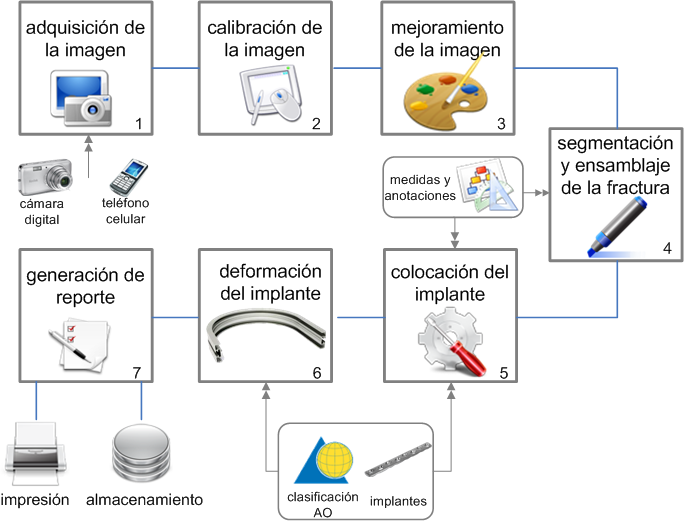
\includegraphics[width=.8\columnwidth]{images/esquema_tesis_mscv4.png}
	\caption{Esquema general de la planificaci\'on preoperatoria digital en Ortopedia}
	\label{fig:esquema}
\end{figure}

El sistema recibe como entrada una imagen correspondiente a una fractura de un paciente, la cual proviene de una placa radiogr\'afica. Una vez adquirida la imagen, se procede a un proceso de calibraci\'on para obtener medidas aproximadas de las proporciones dentro de la imagen (e.g. longitud del hueso en $mm.$). A la imagen calibrada se le puede aplicar t\'ecnicas de mejoramiento como aumento del brillo, contraste, etc., con el objetivo de ayudar en la extracci\'on de los fragmentos de una fractura por parte del traumat\'ologo. Una vez que el traumat\'ologo haya separado los fragmentos de huesos, efect\'ua el ensamblaje del hueso afectado como parte del procedimiento de planificaci\'on.

La fractura tratada puede requerir de un dispositivo externo (placa, tornillo, implante, etc.) para la reducci\'on del hueso. Dicho dispositivo ser\'a seleccionado de un conjunto de plantillas asociadas al tipo de fractura a tratar. Una vez colocado el dispositivo externo, el sistema permite al radi\'ologo aplicar deformaciones dependiendo de la anatom\'ia de la reducci\'on. Al finalizar los pasos antes mencionados, se obtiene el calco necesario para la cirug\'ia y la posibilidad de obtener un reporte con los datos tanto del paciente como del procedimiento a efectuar y su respectivo almacenamiento como parte de la historia cl\'inica del paciente.

Cada uno de los pasos de la Figura \ref{fig:esquema} son explicados con detalle en las secciones a continuaci\'on:

%%%%%%%%%%%%%%%%%%%%%%%%%%%%%%%%%%%%%%%%%%
\subsection{Adquisici\'on de la imagen}

En el modelo propuesto, las im\'agenes se obtienen empleando una c\'amara digital. El procedimiento consiste en los siguientes pasos:
\begin{enumerate}
	\item El m\'edico coloca sobre un negatoscopio la(s) placa(s) de Rayos-X para generar el contraste adecuado.
	\item Se procede a tomar la fotograf\'ia de la placa.
	\item Se descarga la imagen (en formato JPG, BMP, PNG o GIF) al computador.
\end{enumerate}
En la Figura \ref{fig:adquisicion} se ilustra la manera en que debe ser tomada una fotograf\'ia de una placa de Rayos-X. La c\'amara se coloca a una distancia de 1 m. $\pm$ 10 cm. de manera frontal tal que el \'angulo de visi\'on formado por la c\'amara ocupe toda la placa.
\begin{figure}[htb]
	\centering
	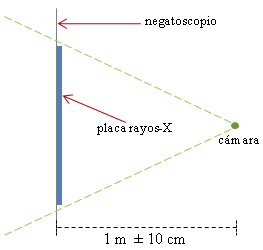
\includegraphics[width=0.4\columnwidth]{images/distancia_ch4.png}
	\caption{Esquema de adquisici\'on de la imagen empleando una c\'amara digital sobre la placa de Rayos-X colocada sobre un negatoscopio}
	\label{fig:adquisicion}
\end{figure}

La resoluci\'on de la fotograf\'ia debe ser de al menos $800 \times 600$ p\'ixeles. Para obtener la resoluci\'on m\'inima requerida de $800 \times 600$, se precisa de una c\'amara de al menos 0.5 megap\'ixeles. N\'otese que la resoluci�n en p\'ixeles cambia de una c\'amara a otra, de acuerdo a su capacidad de captura. Por ejemplo, al tomar una fotograf\'ia de una placa de un f\'emur de un infante se puede obtener la imagen a una resoluci\'on de $1024 \times 768$ p\'ixeles, pero al utilizar una c\'amara distinta y tomar la fotograf\'ia sobre la misma placa se puede obtener una resoluci\'on de $1680 \times 1050$ p\'ixeles.

Conocer las dimensiones reales de una imagen es relevante ya que permitir\'a realizar medidas sobre la misma. Las medidas realizadas sobre la anatom\'ia de un paciente permiten obtener las dimensiones reales de los segmentos de una fractura, la longitud de los huesos, el \'angulo formado entre dos secciones, etc. En la pr\'oxima secci\'on, se muestran los pasos necesarios para permitir la conversi\'on de p\'ixeles a mil\'imetros de la imagen de estudio en un proceso llamado calibraci\'on de la imagen.

%%%%%%%%%%%%%%%%%%%%%%%%%%%%%%%%%%%%%%%%%%
\subsection{Calibraci\'on de la imagen}

La calibraci\'on de la imagen consiste en realizar la correspondencia p\'ixel-mil\'imetro y de esta manera poder realizar medidas sobre la imagen a trabajar en la planificaci\'on. Una soluci\'on com\'un para la calibraci\'on en procesos donde se digitalizan placas de Rayos-X, es la introducci\'on de un objeto de tama\~no conocido al momento de la adquisici\'on de la misma (OR - Objeto de Referencia). Entonces, el proceso de calibraci\'on consiste en definir un Objeto de Referencia que sea utilizado en todos los casos de adquisici\'on de la imagen. Con el OR, se puede calcular un factor de correspondencia p\'ixel-mil\'imetro el cual se utilizar\'a para realizar las medidas correspondientes. En la presente secci\'on se muestran los pasos para la ejecuci\'on de esta etapa.

%%%%%%%%%%%%%%%%%%%%%%%%%%%%%%%%%%%%%%%%%%
\subsubsection{Preparaci\'on de la imagen}

En el esquema propuesto, se utiliz\'o como Objeto de Referencia una perforadora de papel, v\'ease la Figura \ref{fig:paper-punch}. La elecci\'on de este dispositivo de oficina se bas\'o en la necesidad de utilizar un OR que sea disponible en todo momento y pueda estar presente en el momento de la toma independientemente del negatoscopio a utilizar (e.g. negatoscopio general, port\'atil, de mural, etc.).
\begin{figure}[htb]
	\centering
		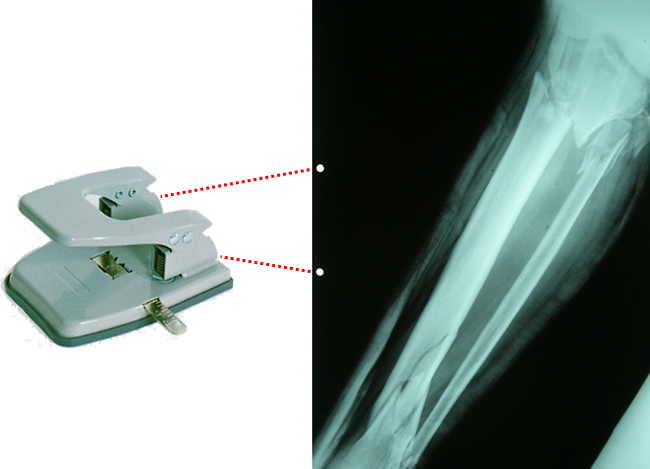
\includegraphics[width=0.4\columnwidth]{images/paperpunch.png}
	\label{fig:paper-punch}
	\caption{Perforadora de papel para crear los orificios en una placa de Rayos-X}
\end{figure}

Dado que la perforadora de papel siempre crea los orificios en los bordes de la placa, solamente se consideran las franjas dentro de la placa donde posiblemente se encuentren \'estas. Entonces, por cada imagen se extraen cuatro (4) subim\'agenes, como se observa en la Figura \ref{fig:paperholes}, para ser analizadas y encontrar los orificios: la parte superior, inferior, derecha e izquierda de la imagen. Para el caso de las subim\'agenes superior e inferior, el ancho corresponde al ancho de la imagen y el alto es de $10\%$ del alto de la imagen original. Se procede de manera similar para las subim\'agenes derecha e izquierda.
\begin{figure}[htb]
	\centering
		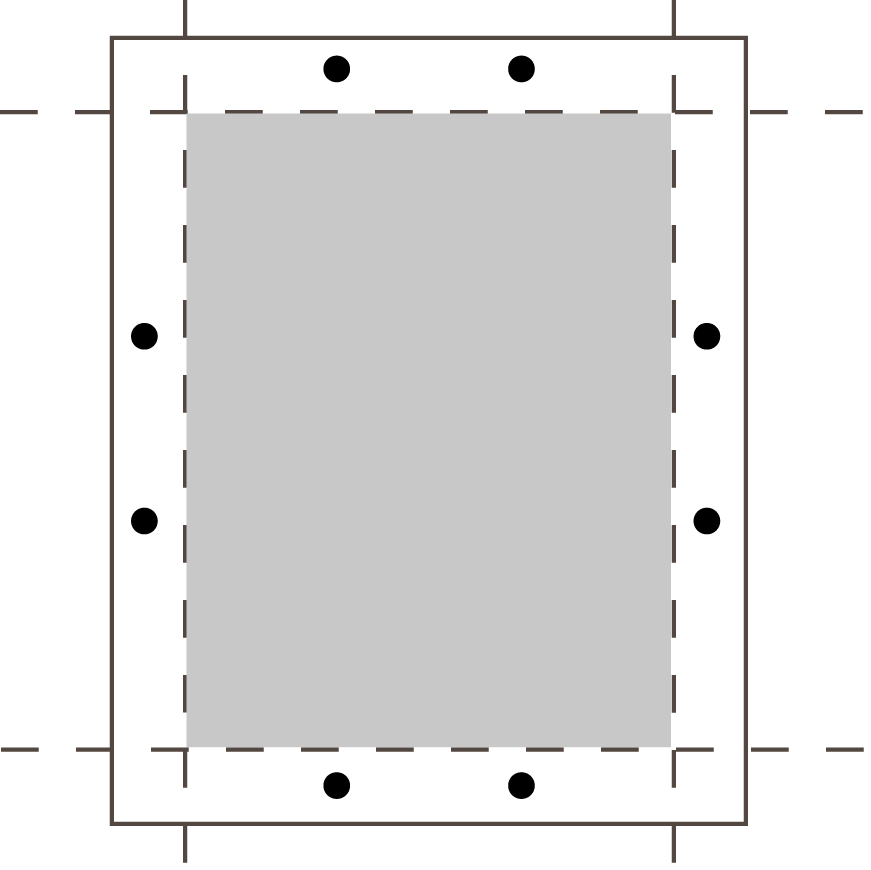
\includegraphics[width=0.4\columnwidth]{images/paperholes.png}	
	\caption{Cuatro (4) posibles franjas donde se abren los orificios con la perforadora de papel}
	\label{fig:paperholes}
\end{figure}

Para cada una de las subim\'agenes, se ejecuta el Algoritmo de B\'usqueda de Orificios y luego el proceso de Calibraci\'on. A continuaci\'on, se explica dicho algoritmo.

%%%%%%%%%%%%%%%%%%%%%%%%%%%%%%%%%%%%%%%%%%
\subsubsection{Algoritmo de B\'usqueda de Orificios} \label{AlgBusqOri1}

El Algoritmo de B\'usqueda de Orificios permite dada una Imagen $I$ de entrada, dos umbrales $U,T$ y un valor de error $E$, determinar la ubicaci\'on de los dos orificios, creados por la perforadora de papel, dentro de $I$. Cabe destacar que el algoritmo requiere como entrada una imagen binaria, es decir, que utilice un solo bit por p\'ixel en su representaci\'on. De esta forma solo existen dos colores: blanco y negro. Se asume que los c\'irculos a buscar ser\'an de color blanco por el contraste generado por el negatoscopio con la placa. Para obtener la imagen binaria, se realiza un proceso de segmentaci\'on a dos niveles de $I$ (\textit{image binarization}). Luego de la binarizaci\'on el algoritmo busca una serie de candidatos a c\'irculos que son colocados en una cola de prioridad bajo un criterio de similitud. Seguidamente, los elementos de la cola son extra\'idos y comparados entre s\'i para encontrar los de mayor similitud entre s\'i.

%%%%%%%%%%%%%%%%%%%%%%%%%%%%%%%%%%%%%%%%%%
\paragraph{Segmentaci\'on a dos niveles}

Con la segmentaci\'on a dos niveles, dada una imagen $I$ se quiere transformar $I$ en una nueva imagen con solo dos colores (e.g. blanco y negro). En el esquema propuesto, la imagen de entrada es a color, como se muestra en la Figura \ref{fig:segBW1}. Esta imagen es convertida a una imagen de 8-bits con paleta de colores, como se observa en la Figura \ref{fig:segBW2}.
\begin{figure}[htb]
  \begin{center} 
  \subfigure[]{\label{fig:segBW1}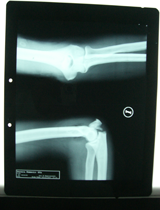
\includegraphics[width=0.30\columnwidth]{images/segmentationBW1.png}} \hspace{0.3cm} 	\subfigure[]{\label{fig:segBW2}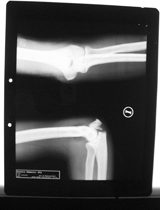
\includegraphics[width=0.30\columnwidth]{images/segmentationBW2.png}} \hspace{0.3cm}
  \subfigure[]{\label{fig:segBW3}
\includegraphics[width=0.30\columnwidth]{images/segmentationBW3.png}}
  \end{center}
  \caption{Etapas de conversi\'on de la imagen original a solo dos niveles de color. (a) Imagen RGB (b) Imagen en niveles de grises (c) Imagen binaria}
  \label{fig:segmentation}
\end{figure}

La conversi\'on de una imagen a color a una imagen a escala de grises se realiza empleando la Ec. \ref{eq:togray}, bajo el criterio explicado en \cite{UMB05}. Con esta ecuaci\'on se obtiene un valor $color_{gray}$ para cada p\'ixel, que representa la intensidad del p\'ixel (dentro del rango $0-255$), bas\'andose en la informaci\'on de cada banda de color de dicho p\'ixel en la imagen original: rojo ($R$), verde ($G$) y azul ($B$).
\begin{equation}
	\label{eq:togray}
	color_{gray} = 0.299 \times R + 0.587 \times G + 0.114 \times B
\end{equation}

Finalmente para obtener la imagen binaria $I_b$, como se muestra en la Figura \ref{fig:segBW3}, se realiza una umbralizaci\'on simple sobre el rango $[200-220]$. El valor adecuado dentro de ese rango, se selecciona de acuerdo a la proporci\'on del color negro en la imagen. Dicho rango fue seleccionado por ser satisfactorio sobre diversas im\'agenes de prueba.

%%%%%%%%%%%%%%%%%%%%%%%%%%%%%%%%%%%%%%%%%%
\paragraph{Algoritmo} \label{AlgBusqOri2}

Una vez obtenido $I_b$ se procede a realizar la b\'usqueda de los orificios. Los orificios creados por la perforadora de papel est\'an aproximadamente a la misma distancia del borde de la placa, es decir, un orificio se encuentra en el mismo sentido vertical u horizontal del otro. Este aspecto es importante al momento de determinar la similitud entre dos posibles orificios detectados por el algoritmo.

El algoritmo de B\'usqueda de Orificios, mostrado en el Algoritmo \ref{busqueda}, selecciona una serie de candidatos a c\'irculos y los coloca en una cola de prioridad. Los candidatos son seleccionados por la similitud entre s\'i para luego seleccionar los candidatos m\'as similares entre s\'i y de esa forma obtener los orificios.

\begin{algorithm}[htbp]
	\caption{B\'usqueda de Orificios}\label{busqueda}
	\begin{algorithmic}[1]
	\Procedure{FindCircles}{$I_b,U,T,E$}	\label{prototype}\Comment{$I_b$ = imagen; U,T = umbral; E = error permitido}
		\For {cada fila $F$ en $I_b$}	\label{first_for}
			\For {cada p\'ixel $P(x,f)$ de color blanco en $F$}
				\State $pN \gets pS \gets pE \gets pO \gets 0$	\Comment{\# de p\'ixeles blancos en direcci\'on Norte, Sur, Este y Oeste}
				\Loop
					\If{$P(x,f+1) = blanco$}
						$pN \gets pN + 1$
					\EndIf
					\If{$P(x,f-1) = blanco$}
						$pS \gets pS + 1$
					\EndIf
					\If{$P(x+1,f) = blanco$}
						$pE \gets pE + 1$
					\EndIf
					\If{$P(x-1,f) = blanco$}
						$pO \gets pO + 1$
					\EndIf
				\EndLoop
				\If{$p\{N|S|E|O\} > 0$ \underline{y} $|((pN+pS)/2) - ((pE+pO)/2)| < U$}
					\State $d_1 = |pS - pN|$
					\State $d_2 = |pE - pO|$
					\If{$|d_1 - d_2| \le T$}
					\Comment{posiblemente $P(x,f)$ es el centro de un c\'irculo}
						\State $Mask \gets \Call{CreateMask}{(pN+pS)/2}$
						\State $error \gets \Call{ECM}{Mask, I_b, P(x,f)}$
							\If{$error \le E$}
								\State $Priority\_Queue.Add(P(x,f), (pN+pS)/2)$
							\EndIf
					\EndIf
				\EndIf
			\EndFor
		\EndFor
		\State $C_1,C_2 \gets \Call {Find2MostSimilar}{Priority\_Queue}$
	\State \textbf{return} $C_1,C_2$\Comment{$C_1$ y  $C_2$ son los orificios hechos por la perforadora}
	\EndProcedure
	\end{algorithmic}
\end{algorithm}

El algoritmo empieza recorriendo cada p\'ixel de color blanco de cada fila de la subimagen que contiene al candidato, con el objetivo de determinar cu\'al es la distancia hasta los bordes de ese posible candidato. Con estos valores, la idea es determinar cu\'al de \'estos es sim\'etrico con respecto a un p\'ixel centro de c\'irculo. Se puede observar que la Figura \ref{fig:circles1} es m\'as irregular en proporci\'on a la distancia a sus bordes desde el centro que la Figura \ref{fig:circles2}. Cabe destacar, que la Figura \ref{fig:circles1} no entra como candidato de orificio en el algoritmo.
\begin{figure}[htb]
  \begin{center} \subfigure[]{\label{fig:circles1}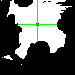
\includegraphics[width=0.20\columnwidth]{images/circles1.png}} \hspace{1.1cm} \subfigure[]{\label{fig:circles2}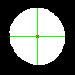
\includegraphics[width=0.20\columnwidth]{images/circles2.png}}
  \end{center}
  \caption{Recorrido en cuatro direcciones para una posici\'on $(x,y)$ de un posible candidato. (a) Forma irregular (b) Forma de orificio}
  \label{fig:circles}
\end{figure}

Para determinar el factor de simetr\'ia de un candidato, se verifica si la distancia desde el centro hacia las cuatro direcciones cardinales tienen longitudes similares. Estas distancias son almacenadas en las variables $pN,pS,pE,pO$ que se muestran en el Algoritmo de B\'usqueda de Orificios y se pueden observar en la Figura \ref{fig:circulo}. 
\begin{figure}[htb]
	\centering
		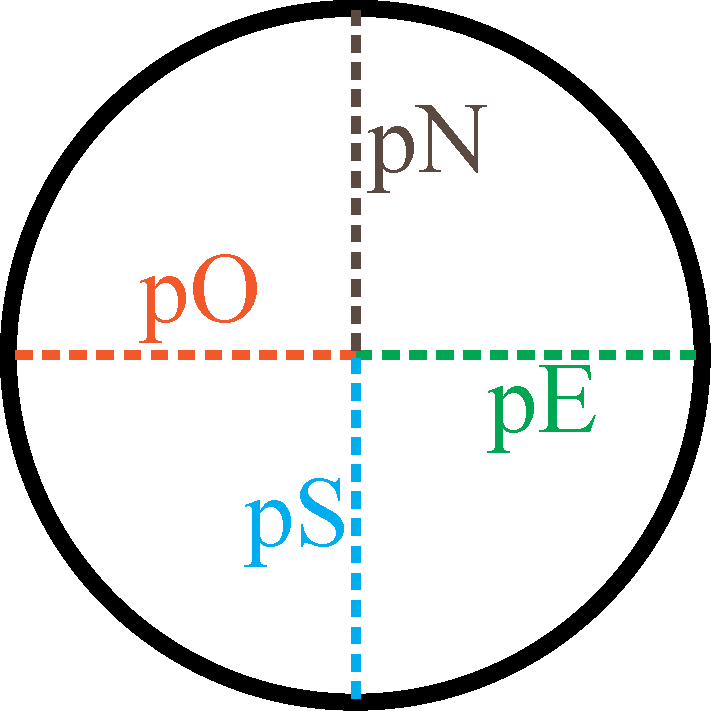
\includegraphics[width=0.25\columnwidth]{images/circle.png}
	\caption{Posible candidato a c\'irculo donde se identifican las 4 distancias obtenidas desde el centro del mismo.}
	\label{fig:circulo}
\end{figure}

Al realizar est\'a operaci\'on en cada p\'ixel de cada fila, permite que se utilicen los valores antes mencionados para el siguiente p\'ixel a analizar. Por ejemplo, si estamos en la posici\'on $(x,y)$ al avanzar a la posici\'on $(x+1,y)$ es ideal utilizar los valores $pN,pS,pE,pO$ de $(x,y)$ para no calcularlos nuevamente.

Para ello se construye una estructura de datos que consiste en un arreglo del tama\~no de una fila donde cada celda almacena 4 valores: $pN,pS,pE,pO$. Con esta estructura, para los valores $pE,pO$ de una posici\'on $(x,y)$ se utilizan sus adyacentes. Cuando se recorre una fila nueva, es decir, la fila $(x,y+1)$, los valores $pN,pS$ son copiados como valores iniciales si existe un p\'ixel blanco en esa posici\'on con el objetivo de no contarlos nuevamente.

Con los valores $pN,pS,pE,pO$ es posible determinar si una posici\'on $(x,y)$ es el centro de un candidato a orificio basados en los valores de umbral $U,T$. El valor umbral $U$ es la diferencia permitida entre el alto y el ancho promediado de un candidato. Dicho valor va a permitir descartar candidatos que su eje vertical/horizontal sea muy distinto al eje contrario. Es por ello que la verificaci\'on dentro del Algoritmo \ref{busqueda} se hace como $\frac{pN+pS}{2} - \frac{pO+pE}{2} < U$. El valor umbral $T$ es la diferencia entre la longitud de los di\'ametros de un posible candidato en forma de c\'irculo. El valor ideal de esta diferencia, debe ser $0$. Este valor permite discriminar candidatos que sean muy ovalados y filtrar los que sean m\'as redondos.

Luego, se invoca a la funci\'on \verb+CreateMask+ donde se construye un arreglo bidimensional que contiene blancos y negros, donde los p\'ixeles blancos forman un c\'irculo, con el objetivo de hacer una coincidencia de patrones \cite{PAJ01} (\textit{pattern matching}) de un espacio dentro de la imagen con un c\'irculo perfecto.

Al realizar la coincidencia de patrones, se calcula el error cuadr\'atico medio \cite{LEH98} con la funci\'on \verb+ECM+. Dicho valor de error permite determinar qu\'e tan parecido es un posible candidato a un c\'irculo perfecto. Si el valor de este error es inferior a cierto umbral $E$, entonces es considerado como un candidato potencial. En las pruebas realizadas, se tomo como valor $E$ un $12\%$ de discrepancia ya que permite considerar los casos en donde la imagen de entrada no sea de buena calidad. Posteriormente, dicha posici\'on $(x,y)$ con un radio de dimensi\'on $(pN+pS)/2$ es insertada en una cola de prioridad. En dicha cola la mayor prioridad la tiene el candidato con menor error $E$.

Como \'ultimo paso del algoritmo, se invoca a la funci\'on \verb+Find2MostSimilar+ que recibe como par\'ametro a la cola de prioridad y busca el par de candidatos de mayor similitud. Los criterios para decidir la similitud son:
\begin{itemize}
	\item Si el candidato $C_1$ ocupa un \'area $A_1$ en p\'ixeles, entonces el candidato $C_2$ tendr\'a una \'area $A_2$ en el rango $A_1 - (0.2*A_1) \le A_2 \le A_1 + (0.2*A_1)$.
	\item Si un candidato se encuentra a una distancia $dx$ del borde de la imagen, el otro candidato debe estar a una distancia $d \le dx*1.5$ del mismo borde.
	\item La distancia entre ambos candidatos, debe ser mayor al $15\%$ del total del lado donde se encuentran (lado horizontal o lado vertical) en la imagen.
\end{itemize}

Finalmente, es posible haber obtenido un solo orificio, dos orificios \'o ninguno. En caso de no haber obtenido ning\'un orificio o solamente uno, se provee la opci\'on de seleccionar el(los) orificio(s) faltante(s) de forma manual. En el caso de haber encontrado ambos orificios, se procede a la calibraci\'on.

%%%%%%%%%%%%%%%%%%%%%%%%%%%%%%%%%%%%%%%%%%
\paragraph{Correspondencia}

Una vez obtenidos ambos orificios, el proceso de calibraci\'on es trivial. Seg\'un el est\'andar ISO (\textit{International Organization for Standardization}) 838 \cite{REF_ISO838} publicado en 1974, titulado ``\textit{Paper $--$ Holes for general filing purposes}'', la distancia entre los centros de cada orificio tiene una medida de $80 \pm 0.5 mm$.

Utilizando el est\'andar, es posible definir est\'a medida como la calibraci\'on para cualquier imagen. Si la distancia entre los centros de los orificios corresponde a $p$ p\'ixeles, entonces $p = 80mm$. Entonces, un p\'ixel corresponde a $\frac{80}{p} mm$. Existen fabricantes de perforadores de orificios que no utilizan el est\'andar ISO en la fabricaci\'on de los mismos y este hecho ocasionar\'ia una calibraci\'on incorrecta. Una soluci\'on a este problema, es ofrecer la posibilidad de modificar la distancia entre orificios de acuerdo al perforador de papel que se utilice, por ejemplo $79.5mm.$, $75mm.$, $81mm.$, etc.

%%%%%%%%%%%%%%%%%%%%%%%%%%%%%%%%%%%%%%%%%%
\subsection{Mejoramiento de la imagen}

Una vez calibrada la imagen, el m\'edico radi\'ologo tiene la posibilidad de modificar ciertos valores visuales dentro de la imagen para mejorar la calidad visual de la misma. Dado que las im\'agenes son de 8-bit, esto permite crear un histograma de frecuencias en el rango de valores $[0-255]$. Dentro de ese rango se pueden definir dos caracter\'isticas empleadas para el mejoramiento: Ventana (\textit{window}) y Nivel (\textit{level}). El \textit{window} define el tama\~no de un rango de valores consecutivos dentro del histograma. El \textit{level} define un valor dentro del rango de valores de la imagen. Con estos valores, es posible definir el valor m\'inimo y m\'aximo de p\'ixel de un rango de datos, al que llamaremos ``ventana''. Si $V_{max}$ define el valor m\'aximo y $V_{min}$ el m\'inimo, entonces $V_{min}=level - \frac{window}{2}$ y $V_{max}=level + \frac{window}{2}$. En la Fig. \ref{fig:window} se muestra un histograma donde se indica el ancho de la ventana demarcado por unas l\'ineas punteadas.
\begin{figure}[htbp]
	\centering
	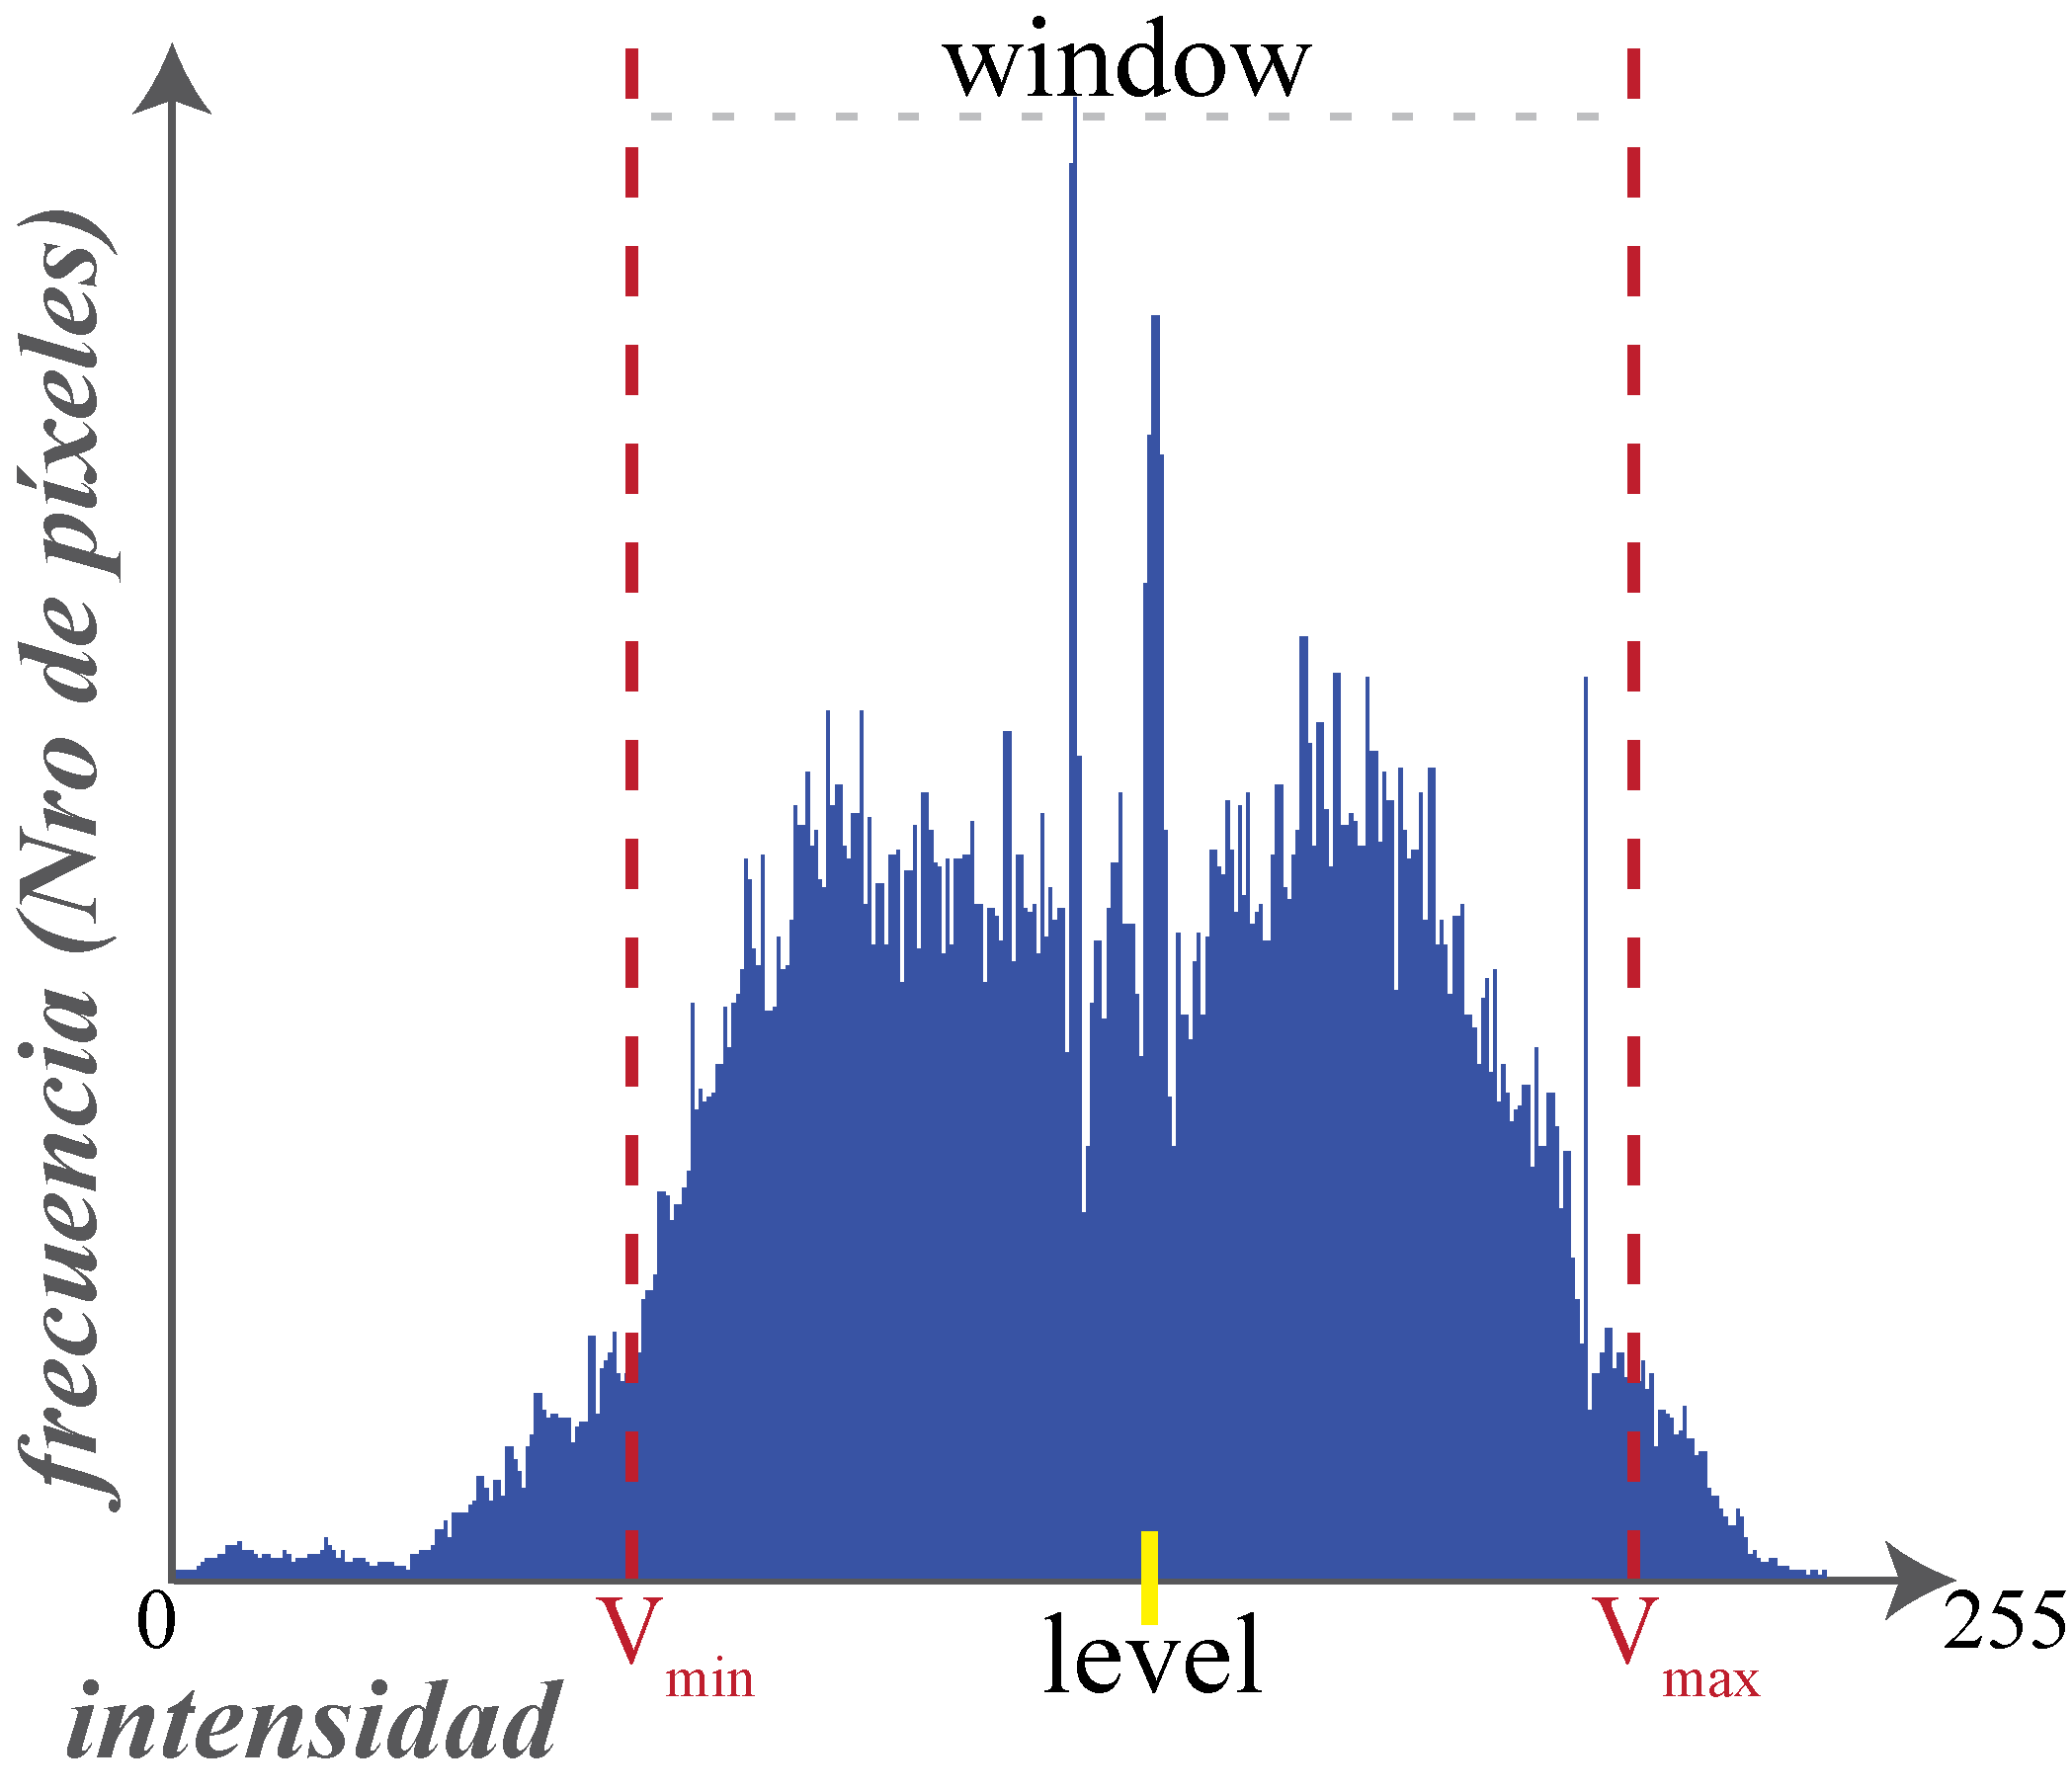
\includegraphics[width=0.5\columnwidth]{images/histograma.png}
	\caption{Histograma de intensidades que muestra el \textit{window} y \textit{level} dentro del histograma.}
	\label{fig:window}
\end{figure}

Por defecto, los valores de \textit{window} y \textit{level} son $255$ y $128$ respectivamente, para que la ventana ocupe todo el rango de valores de la imagen. Sin embargo, ajustando los valores de \textit{window} y \textit{level}, se puede modificar el contraste de la imagen. Por ejemplo, al definir el valor $W = 200$ y $L = 110$, todos los p\'ixeles con una intensidad $I \le 10$ ser\'an llevados a 0, y todos los p\'ixeles con una intensidad $I \ge 210$ ser\'an llevados a 255. Los p\'ixeles con intensidades entre $10$ y $210$ ser\'an mapeados linealmente al rango de valores de salida, que es de $[0,255]$.

En la Figura \ref{fig:mejoramiento1} se muestra una imagen adquirida de un estudio de un paciente luego de ser calibrada. En la Figura \ref{fig:mejoramiento2} se muestra la misma imagen pero con valores de \textit{window} $W=100$ y \textit{level} $L=128$. Por otra parte, en la Figura \ref{fig:mejoramiento3} se tienen los valores $W=255$ y $L=240$. El m\'edico es el encargado de manipular estos valores con el objetivo de obtener un mejor contraste en la imagen para poder realizar la reducci\'on de la fractura en la planificaci\'on.
\begin{figure}[htbp]
  \begin{center}
    \subfigure[]{\label{fig:mejoramiento1}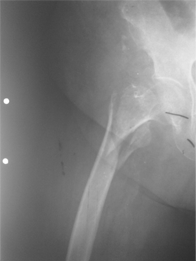
\includegraphics[width=0.30\columnwidth]{images/mejoramiento1.png}} \hspace{0.4cm} \subfigure[]{\label{fig:mejoramiento2}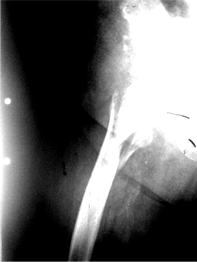
\includegraphics[width=0.30\columnwidth]{images/mejoramiento2.png}} \hspace{0.4cm}  \subfigure[]{\label{fig:mejoramiento3}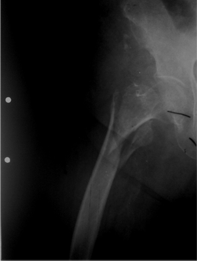
\includegraphics[width=0.30\columnwidth]{images/mejoramiento3.png}}
  \end{center}
  \caption{Mejoramiento de la imagen con diversos valores de \textit{window} y \textit{level} (a) $W=255$ y $L=128$ (b) $W=100$ y $L=128$ (c) $W=255$ y $L=240$}
  \label{fig:mejoramiento}
\end{figure}

Adicionalmente, se ofrece una opci\'on sugerida de contraste basado en la cantidad de intensidades presentes en la imagen. Dicha opci\'on consiste en asignar valores de \textit{window} y \textit{level} tal que la imagen muestre valores relevantes en el contraste adecuado. Para ello se calcula de intensidad promedio de la imagen $I_{average}$. Al mismo tiempo, se calcula el valor de $N_p$ que representa el n\'umero de p\'ixeles que est\'an por encima de $I_{average}$. Finalmente se ubica el valor de \textit{level} en el valor medio del rango de intensidades de la imagen y el valor del \textit{window} es $N_p$.

%%%%%%%%%%%%%%%%%%%%%%%%%%%%%%%%%%%%%%%%%%
\subsection{Segmentaci\'on y ensamblaje de la fractura}

Para efectuar la reducci\'on de una fractura se requiere extraer los fragmentos de hueso presente. Una vez seleccionados los fragmentos, el traumat\'ologo debe ensamblarlos y colocarlos en sus posiciones correctas y as\'i completar la reducci\'on de la fractura.

La selecci\'on de los fragmentos de la fractura en la imagen, requiere un proceso de segmentaci\'on \cite{UMB05} donde se separen dichos fragmentos del hueso a tratar. Los algoritmos existentes para la segmentaci\'on autom\'atica de im\'agenes de Rayos-X no son triviales ya que no existe un procedimiento est\'andar para su ejecuci\'on. En la literatura existen diversas t\'ecnicas para la segmentaci\'on de im\'agenes m\'edicas \cite{HARA85,PAL93,PHAM00} entre las que destacan: los modelos deformables \cite{KASS88,TER87,TER88}, las plantillas deformables param\'etricas \cite{YUI92}, los modelos de distribuci\'on de puntos \cite{COOT94}, las plantillas gr\'aficas \cite{AMIT96} y las plantillas basadas en esqueletos \cite{PIZ98,PIZ99}, entre otras t\'ecnicas. Dichas t\'ecnicas no son 100\% efectivas para todas las im\'agenes. Para conseguir una segmentaci\'on adecuada por lo general se emplean varias de \'estas t\'ecnicas y/o se aplican modificaciones acorde a la imagen en cuesti\'on.

Otra forma de extracci\'on de fragmentos es emplear la segmentaci\'on manual, la cual consiste en delinear los bordes de los fragmentos e ir construyendo un pol\'igono que encierre el fragmento de hueso, como se observa en la Figura \ref{fig:fragmentation}.
\begin{figure}[htb]
  \begin{center} \subfigure[]{\label{fig:segmentation1}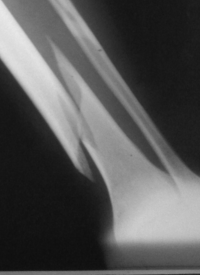
\includegraphics[width=0.25\columnwidth]{images/segmentation1.png}} \hspace{0.5cm} \subfigure[]{\label{fig:segmentation2}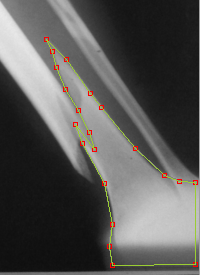
\includegraphics[width=0.25\columnwidth]{images/segmentation2.png}}\hspace{0.5cm} \subfigure[]{\label{fig:segmentation3}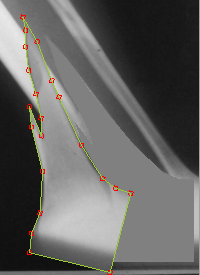
\includegraphics[width=0.25\columnwidth]{images/segmentation3.png}} \hspace{0.5cm}
  \end{center}
  \caption{Segmentaci\'on manual de una fractura donde se seleccionan los fragmentos de hueso para ser colocados en su posici\'on correcta. (a) Fractura simple (b) Pol\'igono que delimita la secci\'on a segmentar (c) Pol\'igono despu\'es de aplicar rotaciones y traslaciones}
  \label{fig:fragmentation}
\end{figure}

En el esquema propuesto se opt\'o por una segmentaci\'on manual. En la Figura \ref{fig:segmentation1} se muestra una fractura simple a ser segmentada por el m\'edico radi\'ologo. En la Figura \ref{fig:segmentation2} se observa una serie de puntos gu\'ia (en color rojo) sobre el contorno del fragmento unidos por una l\'inea formando un pol\'igono irregular. Finalmente, es posible aplicar rotaciones y traslaciones sobre el fragmento con el objetivo de ser colocado en su posici\'on anat\'omicamente correcta para realizar la reducci\'on por parte del radi\'ologo, ver Figura \ref{fig:segmentation3}.

%%%%%%%%%%%%%%%%%%%%%%%%%%%%%%%%%%%%%%%%%%
\subsubsection{Medidas y anotaciones}

Una vez calibrada la imagen es posible realizar mediciones de la anatom\'ia en una imagen empleando diversas herramientas. Las mediciones dentro de una imagen de Rayos-X son importantes para el tratamiento de un paciente, ya que permiten obtener las dimensiones de los segmentos de una fractura, la longitud de los huesos y el \'angulo entre dos secciones (e.g. diferencia entre fragmentos de hueso en una fractura), entre otros. Las medidas son realizadas en $mm.$ y permiten al radi\'ologo definir dimensiones y longitudes \'utiles para su planificaci\'on antes de entrar al quir\'ofano.

Algunas de las herramientas de calibraci\'on se observan en la Figura \ref{fig:medidas}. La Figura \ref{fig:medida1} muestra un tipo de medida denominada \textit{Regla} que consiste en una l\'inea recta que une dos puntos, mostrando la medida en $mm.$ La herramienta denominada \textit{\'Angulo} permite determinar, en grados, el \'angulo existente entre un par de l\'ineas rectas con un punto en com\'un, como se observa en la Figura \ref{fig:medida2}. La \'ultima herramienta de medici\'on se denomina \textit{C\'irculo} y crea un c\'irculo definido por un centro y un di\'ametro, ver Figura \ref{fig:medida3}, la medida es en $mm.$ y viene dada por el valor de su di\'ametro.
\begin{figure}[htb]
  \begin{center}
    \subfigure[]{\label{fig:medida1}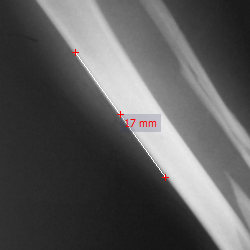
\includegraphics[width=0.35\columnwidth]{images/medirlinea.png}} \hspace{0.55cm} \subfigure[]{\label{fig:medida2}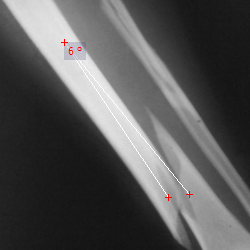
\includegraphics[width=0.35\columnwidth]{images/medirangulo.png}}\hspace{0.55cm}  \subfigure[]{\label{fig:medida3}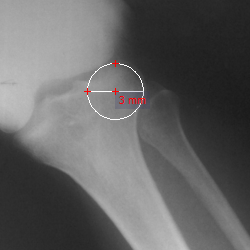
\includegraphics[width=0.35\columnwidth]{images/medircircle.png}} \hspace{0.55cm} \subfigure[]{\label{fig:medida4}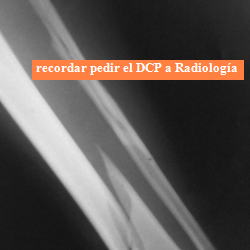
\includegraphics[width=0.35\columnwidth]{images/annotation.png}}
  \end{center}
  \caption{Herramientas de medidas y anotaciones. (a) Regla (b) \'Angulo (c) C\'irculo (d) Anotaci\'on}
  \label{fig:medidas}
\end{figure}

Una funcionalidad sumamente \'util dentro de la planificaci\'on de una operaci\'on son las anotaciones. Las anotaciones permiten colocar informaci\'on de inter\'es dentro de la imagen en formato de texto. Las notas colocadas dentro de la planificaci\'on son libres a juicio del m\'edico radi\'ologo. En la Figura \ref{fig:medida4} se observa un ejemplo de una anotaci\'on. Para facilidad del usuario es posible cambiar el tipo y tama\~no de letra as\'i como el color del fondo del mismo.

%%%%%%%%%%%%%%%%%%%%%%%%%%%%%%%%%%%%%%%%%%
\subsection{Colocaci\'on del implante} \label{IMPLANTE}

Un hueso fracturado debe ser cuidadosamente colocado en la posici\'on adecuada hasta que sea lo suficientemente fuerte como para soportar el peso del paciente, empleando alg\'un tipo de implante. Hasta el siglo pasado \cite{REF_AO}, los m\'edicos se basaron en emplear solamente yesos y f\'erulas para apoyar el hueso por fuera del cuerpo (fijaci\'on externa). Pero el desarrollo en el campo de la cirug\'ia redujo el riesgo de infecci\'on, permitiendo que los m\'edicos puedan trabajar directamente con el hueso y colocar implantes internos (fijaci\'on interna). 

Nuevos materiales tales como acero inoxidable, cobalto y titanio no son solo duraderos, sino que tambi\'en son lo suficientemente fuertes y flexibles para apoyar el hueso. Estos materiales tambi\'en son compatibles con el cuerpo y rara vez causan una reacci\'on al\'ergica en el paciente. Los tipos m\'as comunes de la fijaci\'on son: los alambres, placas, barras, clavijas, pines, clavos y tornillos.

Una vez que se obtienen los segmentos de hueso de una fractura y luego de haber aplicado la reducci\'on de la misma, es decisi\'on del traumat\'ologo la colocaci\'on y selecci\'on de implantes para realizar una fijaci\'on del hueso como parte del tratamiento quir\'urgico. Dependiendo del tipo de fractura, posici\'on anat\'omica y edad del paciente, entre otras variables, se procede a seleccionar el implante adecuado.

El esquema CAOS propuesto, plantea el uso de una librer\'ia \'o repositorio donde se almacenan los diversos implantes. Una librer\'ia de implantes es un conjunto de plantillas (\textit{templates}) de traumatolog\'ia clasificadas bajo alg\'un criterio. De esta forma, se selecciona un tipo de implante (e.g. clavo, placa, etc.), el material del que est\'a hecho y sus dimensiones (e.g. 12mm, 3.5 mm, etc.) para ser colocados en la planificaci\'on preoperatoria a construir.

Una base de datos es una forma de almacenamiento adecuada para colocar la gran cantidad de implantes requeridos para los sistemas CAOS de planificaci\'on preoperatoria. La librer\'ia de implantes utilizada en nuestra propuesta, se muestra como un \'arbol, ver Figura \ref{fig:arbol}, donde cada nivel de jerarqu\'ia indica un orden de acuerdo a la medida, material, tama\~no, etc.
\begin{figure}[htbp]
	\centering
	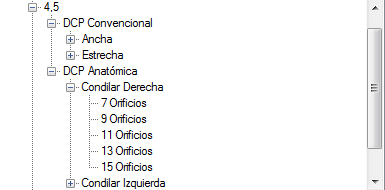
\includegraphics[width=0.5\columnwidth]{images/arbol.png}
	\caption{Vista en forma de \'arbol para representar los implantes de la librer\'ia}
	\label{fig:arbol}
\end{figure}

Una vez seleccionado el implante, \'este se extrae desde un archivo en formato STL (\textit{stereolithography}) generado por el \textit{software} Autodesk Inventor \cite{website:inventor}. En Autodesk Inventor se construye el implante a ser utilizado y es exportado en el formato STL que permite obtener una superficie 3D basada en tri\'angulos.

En el esquema propuesto, el implante seleccionado se muestra como se observa en la Figura \ref{fig:implantproj}, donde se debe seleccionar la orientaci\'on de la vista a utilizar y las dimensiones a emplear.
\begin{figure}[htbp]
	\centering
	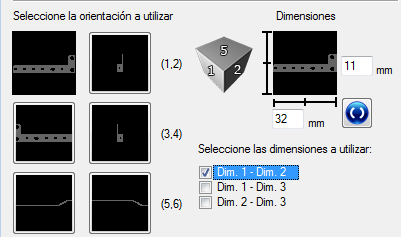
\includegraphics[width=0.60\textwidth]{images/implantprojection.png}
	\caption{Selecci\'on de los par\'ametros necesarios para colocar el implante en la planificaci\'on preoperatoria}
	\label{fig:implantproj}
\end{figure}

Dado que el implante se encuentra representado como una geometr\'ia en 3D, es necesario realizar el proceso de despliegue a 2D. Para ello, se aplica la proyecci\'on ortogonal que consiste en trazar rayos paralelos desde la posici\'on de la c\'amara en direcci\'on hacia el objeto de inter\'es. La posici\'on de la c\'amara se encuentra a una distancia infinita del objeto, resultando que los rayos de visi\'on sean paralelos al plano de proyecci\'on. Los puntos de intersecci\'on de los rayos con el plano de proyecci\'on corresponden al resultado esperado.
\begin{figure}[htbp]
	\centering
	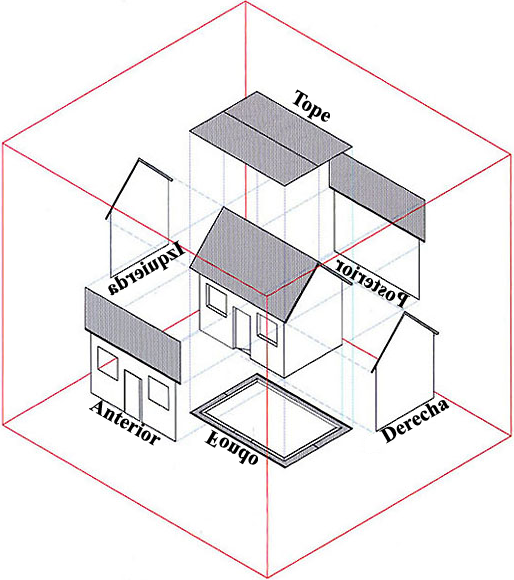
\includegraphics[width=0.35\textwidth]{images/house.png}
	\caption{Proyecci\'on paralela de un objeto casa sobre cada una de las caras de un cubo para obtener 6 proyecciones}
	\label{fig:house}
\end{figure}

En la Figura \ref{fig:house} se muestra un ejemplo de proyecci\'on paralela para un objeto que representa una casa, aplicada sobre cada cara de un cubo. Bajo este esquema, es posible obtener diferentes vistas para un objeto: tope, fondo, derecha, izquierda, anterior y posterior. Al seleccionar un implante en la interfaz propuesta, ver Figura \ref{fig:implantproj}, es posible seleccionar la vista a aplicar para una planificaci\'on. Las vistas se encuentran numeradas del 1 al 6 y adicionalmente se debe escoger las dimensiones a aplicar. Dado que no se conoce a priori la orientaci\'on original del implante (obtenido de Autodesk Inventor \cite{website:inventor}) se provee la opci\'on de seleccionar las dimensiones que representan las distancias que ocupa el implante (ancho, alto y profundidad).

%%%%%%%%%%%%%%%%%%%%%%%%%%%%%%%%%%%%%%%%%%
\subsection{Deformaci\'on del implante} \label{DEFO}

Como vimos anteriormente, los sistemas CAOS deben proveer una librer\'ia de implantes donde el m\'edico cirujano seleccione uno de \'estos para ser colocados en la fractura en cuesti\'on. En muchas ocasiones, es necesario moldear (deformar) el implante tal que sea anat\'omicamente correcto y se adapte al hueso fracturado. 

Dentro del quir\'ofano, el m\'edico cirujano emplea un alicate especial para el doblado de los implantes. En el sistema CAOS propuesto, la deformaci\'on del implante se realiza simulando la aplicaci\'on de una fuerza mec\'anica tal como se realiza en un quir\'ofano. 

En la Figura \ref{fig:tornillo}, se muestra un implante (placa) colocado sobre un f\'emur y su doblado dentro del mismo. Cabe destacar, que el doblado es una tarea exclusiva del m\'edico cirujano y no requiere mucha precisi\'on.
\begin{figure}[htb]
  \begin{center}
 \subfigure[]{\label{fig:tornillo1}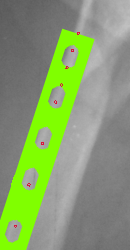
\includegraphics[width=0.23\columnwidth]{images/tornillo1.png}} \hspace{0.15cm} 			\subfigure[]{\label{fig:tornillo2}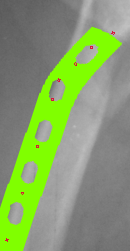
\includegraphics[width=0.23\columnwidth]{images/tornillo2.png}}
  \end{center}
  \caption{Implante de una placa de $4.5$ mm. de comprensi\'on convencional estrecha de 8 orificios sobre una placa de Rayos-X. (a) Sin aplicar deformaci\'on (b) Con una peque\~na deformaci\'on}
  \label{fig:tornillo}
\end{figure}

Tanto en el momento de la colocaci\'on del implante como en el de su deformaci\'on, es posible consultar en una gu\'ia de referencia los tipos de fracturas existentes seg\'un la clasificaci\'on AO. En el siguiente Cap\'itulo, se presentar\'a una descripci\'on m\'as detallada del proceso de deformaci\'on aplicado en nuestro trabajo.

%%%%%%%%%%%%%%%%%%%%%%%%%%%%%%%%%%%%%%%%%%
\subsubsection{Biblioteca de clasificaci\'on AO}

Una vez confirmada la fractura de un paciente, \'esta es localizada y clasificada de acuerdo a un esquema establecido. El esquema de clasificaci\'on de una fractura est\'a especificado de acuerdo a su ubicaci\'on anat\'omica. El esquema de clasificaci\'on utilizado en este trabajo es el AO \cite{REF_AO}.

En el esquema internacional de clasificaci\'on de fracturas AO, el m\'edico traumat\'ologo clasifica una fractura de acuerdo a la ubicaci\'on de la misma y sus caracter\'isticas morfol\'ogicas. AO plantea una clasificaci\'on basada en dos n\'umeros: el primero indica una ubicaci\'on en el cuerpo (1-h\'umero, 2-c\'ubito y radio, 3-f\'emur y 4-tibia y peron\'e) y el segundo, el segmento dentro del hueso (1-proximal, 2-diafisal, 3-distal). Una vez seleccionados ambos n\'umeros, entra en una clasificaci\'on por tipo de fractura (A-simple, B-en cu\~na, C-compleja). Luego, la fractura es dividida en tres grupos que miden la escala de severidad de la misma (1, 2, 3).

Esta clasificaci\'on es utilizada como una gu\'ia para el pron\'ostico y eficiencia en el tratamiento de una fractura. El esquema AO es recomendado internacionalmente porque es cl\'inicamente relevante, sencillo, reproducible y provee una buena estimaci\'on del resultado cl\'inico \cite{MULL90}. 

La biblioteca de referencia que nuestro sistema provee, ayudar\'a considerablemente al m\'edico radi\'ologo para que en cualquier momento pueda consultarla para una determinada fractura. En la Figura \ref{fig:aoexample} se observa la forma como se presenta la biblioteca de clasificaci\'on: a) se selecciona el hueso a estudiar y b) se selecciona la parte de la misma.
\begin{figure}[htbp]
  \begin{center}
    \subfigure[]{\label{fig:aoexample1}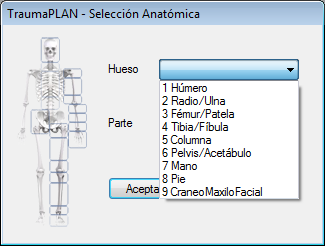
\includegraphics[width=0.45\columnwidth]{images/AOhueso.png}} \hspace{0.15cm} 			\subfigure[]{\label{fig:aoexample2}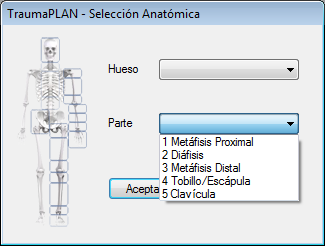
\includegraphics[width=0.45\columnwidth]{images/AOparte.png}}
  \end{center}
  \caption{Biblioteca de clasificaci\'on AO. (a) selecci\'on del hueso a consultar (b) parte dentro del hueso}
  \label{fig:aoexample}
\end{figure}

Una vez seleccionado el hueso y la parte, aparece el tipo de fractura y su severidad. Existe un m\'aximo de 9 clasificaciones posibles para ello, y son mostradas como im\'agenes para su mejor presentaci\'on. Para cada una de las clasificaciones mostradas, se tiene una imagen ejemplo de la fractura, una placa radiogr\'afica con la fractura y una peque\~na descripci\'on de la misma. En la Figura \ref{fig:aoexamplefinal} se puede observar las fracturas de f\'emur en la parte diafisiaria.
\begin{figure}[htbp]
	\centering
	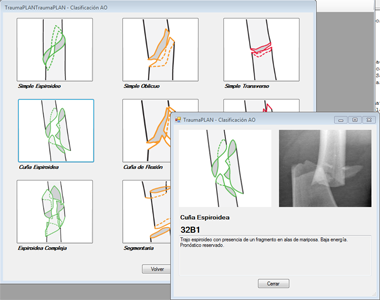
\includegraphics[width=0.50\textwidth]{images/AOexample.png}
	\caption{Clasificaci\'on AO que el sistema provee para una fractura de f\'emur del tipo $32B1$}
	\label{fig:aoexamplefinal}
\end{figure}

%%%%%%%%%%%%%%%%%%%%%%%%%%%%%%%%%%%%%%%%%%
\subsection{Generaci\'on de reporte}

Al realizar el proceso de colocaci\'on de los implantes requeridos para un paciente, se obtiene una imagen que muestra la fractura en cuesti\'on, los implantes, anotaciones y medidas. Con esta informaci\'on, se genera un reporte en formato digital que permita su impresi\'on, env\'io por e-mail, almacenamiento en el sistema PACS, etc.
\begin{figure}[htp]
	\centering
	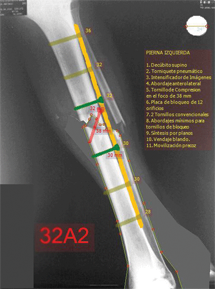
\includegraphics[width=0.4\textwidth]{images/report.png}
	\caption{Reporte generado de reducci\'on de una fractura del tipo 32A2, indicando todos los elementos necesarios para la colocaci\'on de un implante quir\'urgico a un paciente}
	\label{fig:report}
\end{figure}

Un reporte consiste de una imagen seleccionada que incluye implantes, medidas e informaci\'on que describe al paciente y los procedimientos quir\'urgicos que ayudar\'an al m\'edico cirujano durante la cirug\'ia. El texto que aparece en un reporte, se encuentra por encima de la imagen o en una caja de texto (\textit{textbox}), y los implantes a utilizar se deben mostrar claramente, como se observa en la Figura \ref{fig:report}.

La creaci\'on de un reporte de la planificaci\'on permitir\'a tener un resumen de todo el trabajo realizado en el sistema CAOS. El hecho de que el reporte sea digital contribuye a desarrollar la Telemedicina \cite{MEH02}, la cual consiste en la prestaci\'on de servicios de medicina a distancia, particularmente para el diagn\'ostico.

Como \'ultimo paso del proceso, el reporte y la informaci\'on del paciente pueden ser almacenados (el reporte se presenta en formato PDF) para su posterior uso dentro del quir\'ofano, o ser empleado como historia cl\'inica de un caso en particular.